% !TeX root = ../main.tex
% Add the above to each chapter to make compiling the PDF easier in some editors.

\chapter{Aufgabenstellung}
Das Ziel dieses interdisziplinären Projektes der Fakultäten Informatik und Bau Geo Umwelt war es, ein interaktives Werkzeug zu erstellen, mit dem die Ergebnisse einer vergleichenden Ökobilanz für verschiedene Sanierungsvarianten eines Gebäudes visualisiert werden können. Das Tool ist als Teil der Lehr- und Lernplattform „Bilanzlabor“ gedacht, die Studierenden über die Themen Nachhaltigkeit und Lebenszyklusanalyse in anschaulicher Form informieren soll.
\section{Lehr- und Lernplattform Bilanzlabor}
Das Bilanzlabor entstand Ende 2014 als Initiative des Zentrums für nachhaltiges Bauen, einem Zusammenschluss verschiedener Lehrstühle der Fakultäten Bau Geo Umwelt, Architektur sowie Elektro- und Informationstechnik. Die Idee war es, eine Plattform zu erstellen, die basierend auf dem Ansatz der forschungsorientierten Lehre Studierenden die Möglichkeit gibt, sich gesamtheitliche Kenntnisse in den Bereichen Nachhaltigkeit und Lebenszyklusanalyse anzueignen und darüber hinaus hilft die wissenschaftliche Zusammenarbeit der beteiligten Fakultäten auf diesen Gebieten zu stärken. Die Inhalte der Lernplattform sollten dabei sowohl von Seiten der Studierenden als auch von Forschern des Bereichs erstellt und bearbeitet werden können. Um dies zu ermöglichen, ist das Bilanzlabor als Internetseite realisiert, die das quelloffene Enterprise Portal „Liferay Portal“ verwendet. Dieses beinhaltet zum einen ein Content-Management-System zur Organisation von Inhalten, die gemeinschaftlich erstellt und bearbeitet werden können, und zum anderen verschiedene Groupware-Komponenten wie Wikis, Foren und Instant Messaging, welche die gemeinsame Zusammenarbeit unterstützen. Zudem gibt es ein System zur rollenbasierten Autorisierung, um Berechtigungen zu erteilen und zu verwalten. Studierende und Wissenschaftler können sich somit über ihre TUM-Kennung authentifizieren und anschließend je nach Berechtigung verschiedene Inhalte einsehen und/oder bearbeiten. Dies ist ohne Programmierkenntnisse der Benutzer möglich.
\section{Vergleichende Ökobilanz verschiedener Sanierungsszenarien}
Das hier beschriebene Projekt sollte einen Beitrag zum Bilanzlabor leisten, indem es dieses um eine interaktive Visualisierung einer vergleichenden Ökobilanz erweitert. 
\subsection{Datengrundlage (Masterarbeit T. Dzharov)}
Die Daten, die der Visualisierung zu Grunde liegen, stammen aus der Masterarbeit von T. Dzharov. Dort wurde untersucht, wie sich verschiedene Sanierungsszenarien auf die Ökobilanz eines Gebäudes auswirken. Bei dem betrachteten Wohngebäude handelte es sich um ein typisches Projekt aus der Nachkriegszeit (1958) mit ungedämmten Außenwänden sowie dezentralen Niedertemperatur-Gasheizkesseln für die Bereitstellung von Trinkwarmwasser und zur Deckung des Heizbedarfs. Die ehemaligen Fenster mit Holzrahmen waren bereits durch solche mit Kunststoffrahmen und 2-Scheiben-Isolierverglasung ersetzt worden. Die untersuchten Sanierungsvarianten unterschieden sich in Energiestandard, Fenstertyp, Außenwanddämmung, Wärmebrücken und Heizungstechnik. Die Optionen für diese Stellschrauben sind in Tabelle~\ref{tab:layers} aufgelistet. 
 
\begin{table}[htpb]
	\caption[Example table]{Stellschrauben der Gebäudesanierung}\label{tab:layers}
	\centering
	\begin{tabular}{l p{10cm}}
		\toprule
		Stellschraube & Optionen \\
		\midrule
		\multirow{3}{*}{Energiestandard} & EnEv 2016\\
		& KfW70 \\
		& KfW55\\ \hline
	    \multirow{3}{*}{Fenster} & Bestand\\
		& Dena 2-Scheiben WSV \\
		& Dena 3-Scheiben WSV\\ \hline
	    \multirow{3}{*}{Wärmedämmung} & EPS-Dämmung\\
		& Holzfaserdämmung \\
		& Hinterlüftete Fassade mit Mineralwolldämmung\\ \hline
	    \multirow{2}{*}{Wärmebrücken} & Wärmebrückenkorrekturfaktor 0,1\\
		& Wärmebrückenkorrekturfaktor 0,05 \\ \hline
	    \multirow{3}{*}{Heizungstechnik (TGA)} & Zentralheizung mit Gasbrennwertkessel und neuen Radiatoren\\
		& Zentralheizung mit Wärmepumpe Luft/Wasser und Flächenheizung \\
		& Zentralheizung mit Pelletkessel und neuen Radiatoren\\ \hline
		\bottomrule
	\end{tabular}
\end{table}

Zusätzlich wurden einige Sanierungsvarianten mit einer Dachaufstockung analysiert, bei der das Dachgeschoss in die thermische Hülle des Gebäudes eingeschlossen wurde. Auch die Nutzung von Sonnenenergie durch die Installation photovoltaischer beziehungsweise solarthermischer Anlagen wurde untersucht.
Für jede der aus der Kombination der verschiedenen Optionen entstehenden Sanierungsvarianten wurde eine Lebenszyklusanalyse über einen Bilanzierungszeitraum von 30 Jahren erstellt. Der betrachtete Zeitraum richtete sich nach der durchschnittlichen technischen Lebensdauer der Mehrzahl, der bei Sanierungsmaßnahmen verwendeten Bauteile. Die Lebenszyklusphasen für das Produktsystem „Gebäude“ wurden für die Auswertung in die drei größeren Blöcke „Herstellung“, „Nutzung“ und „Rückbau“ zusammengefasst. Die im Rahmen der Wirkungsabschätzung betrachteten Wirkungskategorien sind in Tabelle~\ref{tab:wirkungsindikatoren} zu sehen.

\begin{table}[htpb]
	\caption[Example table]{Betrachtete Wirkungskategorien und ihre Indikatoren}\label{tab:wirkungsindikatoren}
	\centering
	\begin{tabular}{p{7cm} l l}
		\toprule
		Wirkungskategorie & Abkürzung & Wirkungsindikator \\
		\midrule
		Nicht erneuerbare Primärenergie (total) & PENRT & Mega-Joule\\ \hline
		Erneuerbare Primärenergie (total) & PERT & Mega-Joule\\ \hline
		Versauerungspotenzial & AP & kg SO\textsubscript{2}-Äquivalent\\ \hline
		Potenzial für den abiotischen Abbau nicht fossiler Ressourcen & ADPE & kg Sb-Äquivalent\\ \hline
		Treibhauspotenzial & GWP & kg CO\textsubscript{2}-Äquivalent\\ \hline
		Eutrophierungspotenzial & EP & kg PO\textsubscript{4}\textsuperscript{2-}-Äquivalent\\ \hline
		Photochemische Ozonbildung & POCP & kg Ethen-Äquivalent\\ \hline
		Ozonabbaupotenzial & ODP & kg CFC11-Äquivalent\\ \hline
		\bottomrule
	\end{tabular}
\end{table}

\subsection{Ziel der Darstellung im Bilanzlabor}
Die Ergebnisse der vergleichenden Ökobilanz sollten auf der Plattform „Bilanzlabor“ so präsentiert werden, dass Studierenden die Umweltauswirkungen verschiedener Sanierungsmaßnahmen deutlich wird. Trotz der Tatsache, dass es sich bei den erhobenen Daten um die eines spezifischen, wenn auch typischen Wohngebäude der Nachkriegszeit handelt,  sollten sich die qualitativen Resultate durchaus generalisieren lassen. Durch eine Beschränkung auf die Wirkungskategorien PENRT, GWP, AP und ODP, werden nur die eindrücklichsten Unterschiede dargestellt.

\chapter{Umsetzung}
Zur Realisierung des Projektes wurde zunächst, ausgehend von einem von T. Dzharov im Rahmen seiner Masterarbeit entwickelten Entwurfes, die Planung einer interaktiven Benutzeroberfläche durchgeführt. Nach der Analyse der vorhandenen Daten folgte die Konzeption einer geeigneten Programmarchitektur um die benötigten Informationen für die Visualisierung zur Verfügung zu stellen und eine Einbindung in die Plattform „Bilanzlabor“ zu ermöglichen.
\section{Datenaufbereitung}
Als Datenbasis stand pro Sanierungsvariante je eine mit dem Tabellenkalkulationsprogramm Excel erstellte Datei zur Verfügung, die die Berechnung der jeweiligen Ökobilanzierung enthielt. Die Dateinamen richteten sich nach den Ausprägungen der Sanierungsoptionen und weitestgehend im in Abbildung~\ref{fig:dateinamenschema} gezeigten Format angegeben. Da die Abkürzungen für die Optionen teilweise nicht einheitlich verwendet worden waren, bestand der erste Schritt der Datenaufbereitung darin, durch die Umbenennung der Dateien eine automatisierte Zuordnung zwischen einer Kombination von Sanierungsoptionen und der die betreffenden Daten enthaltenden Datei zu gewährleisten.
\begin{figure}[htbp]
	\centering
	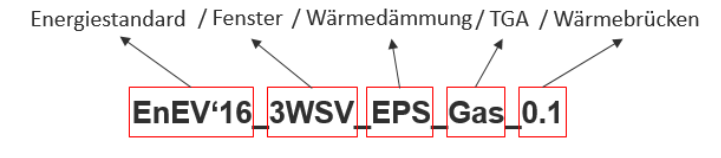
\includegraphics[height=30mm]{figures/dateiname.png}
	\caption[Dateinamenschema]{Dateinamenschema (nach \autocite{milgram})}
	\label{fig:dateinamenschema}	
\end{figure}   
Des Weiteren existierte eine Excel-Datei mit einer Tabelle in der die Ergebnisse der einzelnen Ökobilanzen zusammengefasst aufgeführt waren. Das Schema mit einigen Bespieldaten ist in Tabelle X zu sehen.
\begin{table}[htpb]
	\caption[Example table]{Schema der Tabelle des Sanierungsvariantenvergleichs }\label{tab:wirkungsindikatoren}
	\centering
	\begin{tabular}{l l l l}
		\toprule
		Variante & WK\textsuperscript{*}\_Herstellung & WK\textsuperscript{*}\_Nutzung & WK\textsuperscript{*}\_Rückbau \\
		\midrule
		EnEV'16\_FB\_EPS\_Pellets\_0.1 & 531429.68
		 & 1670135.52 &
		  -195844.54
		  \\ \hline
		\bottomrule
	\end{tabular}
\caption*{\textsuperscript{*} Diese Spalten existieren für jede der Wirkungskategorien PENRT, GWP, ADP und ODP}
\end{table} 
\section{Architektur der Software}
\section{Integration in Liferay}

\chapter{Anwenderdokumentation}

